\documentclass{include/protokollclass}
% Main File - Based on protokollclass.cls
% Comments are mostly in English (and some in German, concerning the Praktikum)
% ------------------------------------------------------------------------------
% Further files in folder:
%  - include/cmds.tex (for macros and additional commands)
%  - include/kitlogo.pdf (for titlepage)
%  - lit.bib (bibtex bibliography database)
%  - include/titlepage.tex (for layout of titelpage)
% ------------------------------------------------------------------------------
% Useful Supplied Packages:
% amsmath, amssymb, mathtools, bbm, upgreek, nicefrac,
% siunitx, varioref, booktabs, graphicx, tikz, multicol





%% ---------------------------------------------
%% |    Informationen über dieses Protokoll    |
%% ---------------------------------------------
\newcommand{\praktikum}{P1}                % P1 oder P2
\newcommand{\semester}{WS21/22}            % z.B. "WS14/15" oder "SS15"

\newcommand{\wochentag}{Do}                % Mo, Di, Mi oder Do
\newcommand{\gruppennr}{7}                % Zweistellige Gruppennummer

\newcommand{\nachnamea}{Linn}             % Nachname des ersten Praktikanten
\newcommand{\vornamea}{Myriel}               % Vorname des ersten Praktikanten
\newcommand{\nachnameb}{Schwartz}           % Nachname des zweiten Praktikanten
\newcommand{\vornameb}{Arne}              % Vorname des zweiten Praktikanten

\newcommand{\emailadressen}{latexvorlage@fachschaft.physik.kit.edu}
% optionale Angabe von Emailadresse(n) für den Kontakt mit dem Betreuer

\newcommand{\versuch}{Aeromechanik} % Name des Versuchs
\newcommand{\versuchsnr}{80}               % bitte die korrekte Nummer dem 
                                           % Arbeitsplatz am Versuchstag 
                                           % entnehmen
\newcommand{\fehlerrechnung}{Nein}         % Ob Fehlerrechnung im Versuch 
                                           % durchgeführt wurde oder nicht

\newcommand{\betreuer}{Florian Schrepp}      % Name des zuständigen Betreuers
\newcommand{\durchgefuehrt}{04.11.21}      % Datum, an dem der Versuch 
                                           % durchgeführt wurde




%% --------------------------------------
%% |    Settings for Word Separation    |
%% --------------------------------------
% Help for separation:
% In German package the following hints are additionally available:
% "- = Additional separation
% "| = Suppress ligation and possible separation (e.g. Schaf"|fell)
% "~ = Hyphenation without separation (e.g. bergauf und "~ab)
% "= = Hyphenation with separation before and after
% "" = Separation without a hyphenation (e.g. und/""oder)

% Describe separation hints here:
\hyphenation
{
    über-nom-me-nen an-ge-ge-be-nen
    %Pro-to-koll-in-stan-zen
    %Ma-na-ge-ment  Netz-werk-ele-men-ten
    %Netz-werk Netz-werk-re-ser-vie-rung
    %Netz-werk-adap-ter Fein-ju-stier-ung
    %Da-ten-strom-spe-zi-fi-ka-tion Pa-ket-rumpf
    %Kon-troll-in-stanz
}





% um die Titelseite per PDF-reader auszufüllen. Vorgefertigte Daten
% können in Datei 'data.tex' modifiziert werden.
%\setboolean{forminput}{true}
% um die Anmerkungen zu den Textfeldern anzeigen zu lassen
%\setboolean{showannotations}{true}
% Erneuern der Seitenzahl in jedem Kapitel
%\setboolean{chapResetPageNumb}{true}
% Einbinden der Kapitelnummer in der Seitenzahl
%\setboolean{chapWiseNumb}{true}
% english or ngerman (new german für neue deutsche Rechtschreibung statt german)
\SelectLanguage{ngerman}





%% -----------------------
%% |    Main Document    |
%% -----------------------
\begin{document}
    % Titlepage und ToC
    \FrontMatter

    % coordinates for background border
\newcommand{\diameter}{20}
\newcommand{\xone}{-15}
\newcommand{\xtwo}{160}
\newcommand{\yone}{15}
\newcommand{\ytwo}{-253}

\newcommand{\hoehea}{55}
\newcommand{\hoeheb}{55}




\begin{titlepage}
    % background border
    \begin{tikzpicture}[overlay]
    \draw[color=gray]  
            (\xone mm, \yone mm)
      -- (\xtwo mm, \yone mm)
    arc (90:0:\diameter pt) 
      -- (\xtwo mm + \diameter pt , \ytwo mm) 
        -- (\xone mm + \diameter pt , \ytwo mm)
    arc (270:180:\diameter pt)
        -- (\xone mm, \yone mm);
    \end{tikzpicture}
    
    % KIT logo
    \begin{textblock}{10}[0,0](4.5,2.5)
        
\includegraphics[width=.25\textwidth]{include/kitlogo.pdf}
    \end{textblock}
    \changefont{phv}{m}{n}    % helvetica
    \begin{textblock}{10}[0,0](5.5,2.2)
        \begin{flushright}
            \Large FAKULTÄT FÜR PHYSIK\\Praktikum Klassische Physik
        \end{flushright}
    \end{textblock}
    
    \begin{textblock}{10}[0,0](4.2,3.1)
        \begin{tikzpicture}[overlay]
        \draw[color=gray]
            (\xone mm + 5 mm, -8 mm)
         -- (\xtwo mm + \diameter pt - 5 mm, -8 mm);
        \end{tikzpicture}
    \end{textblock}
    
    \Large
    % Zeile 1
    \begin{textblock}{12}[0,0](3.58,4)
        \mytextfield{Prak.}{\praktikum}{0.9cm}{17pt}
                    {P1/P2}{2}{Praktikum}
    \end{textblock}
    \begin{textblock}{12}[0,0](5.53,4)
        \mytextfield{Semester}{\semester}{2.6cm}{17pt}
        {z.B. \glqq WS14/15\grqq\ oder \glqq SS15\grqq}{0}{Semester}
    \end{textblock}
    \begin{textblock}{12}[0,0](9.53,4)
        \mytextfield{Wochentag}{\wochentag}{1.3cm}{17pt}
                    {Mo/Di/Mi/Do}{2}{Wochentag}
    \end{textblock}
    \begin{textblock}{12}[0,0](12.88,4)
       \mytextfield{Gruppennr.}{\gruppennr}{1.06cm}{17pt}
                   {\#\#}{2}{Gruppennummer}
    \end{textblock}
    
    % Zeile 2
    \begin{textblock}{12}[0,0](3.58,4.55)
        \mytextfield{Name}{\nachnamea}{6cm}{17pt}
                    {}{0}{Name1}
    \end{textblock}
    \begin{textblock}{12}[0,0](9.53,4.55)
        \mytextfield{Vorname}{\vornamea}{6cm}{17pt}
                    {}{0}{Vorname1}
    \end{textblock}
    
    % Zeile 3
    \begin{textblock}{12}[0,0](3.58,5.1)
        \mytextfield{Name}{\nachnameb}{6cm}{17pt}
                    {}{0}{Name2}
    \end{textblock}
    \begin{textblock}{12}[0,0](9.53,5.1)
        \mytextfield{Vorname}{\vornameb}{6cm}{17pt}
                    {}{0}{Vorname2}
    \end{textblock}
    
    % Zeile 4
    \begin{textblock}{12}[0,0](3.64,5.65)
       \normalsize\mytextfield{Emailadresse(n)}{\emailadressen}{13.1cm}{10pt}
                              {Optional}{0}{Emailadressen}
    \end{textblock}
    
    % Zeile 5
    \begin{textblock}{12}[0,0](3.58,6.2)
        \mytextfield{Versuch}{\versuch\ (\praktikum-\versuchsnr)}{9.45cm}{14pt}
                    {z.B. \glqq Galvanometer (P1-13)\grqq\ oder \glqq %
                     Mikrowellenoptik (P2-15)\grqq}{0}{Versuch}
    \end{textblock}
    \begin{textblock}{12}[0,0](12.58,6.2)
       \mytextfield{Fehlerrech.}{\fehlerrechnung}{1.46cm}{17pt}
                   {Ja/Nein}{4}{Fehlerrechnung}
    \end{textblock}
    
    % Zeile 6
    \begin{textblock}{12}[0,0](3.58,6.75)
        \mytextfield{Betreuer}{\betreuer}{7cm}{17pt}{}{0}{Betreuer}
    \end{textblock}
    \begin{textblock}{12}[0,0](10.82,6.75)
        \mytextfield{Durchgeführt am}{\durchgefuehrt}{2.53cm}{17pt}
                    {TT.MM.JJ}{8}{Durchfuehrung}
    \end{textblock}
    
    % Querstrich
    \begin{textblock}{20}[0,0](0,7.1)\tiny\centering
        Wird vom Betreuer ausgefüllt.
    \end{textblock}
    \begin{tikzpicture}[overlay]
    \draw[color=gray]
        (\xone mm + 5 mm, -78 mm)
     -- (\xtwo mm + \diameter pt - 5 mm, -78 mm);
    \end{tikzpicture}
    
    % Zeile 1
    \begin{textblock}{12}[0,0](3.58,8)
        \myTtextfield{1. Abgabe am}{}{2.5cm}{17pt}
                     {}
    \end{textblock}
    \begin{textblock}{20}[0,0](8.3,8)
        \myTtextfield{Rückgabe am}{}{2.5cm}{17pt}
                     {}
    \end{textblock}
    
    % Block 1
    \begin{tikzpicture}[overlay]
    \draw[color=gray]  
        (\xone mm + 10 mm, -85.5 mm)
     -- (\xtwo mm + \diameter pt - 10 mm, -85.5 mm)
     -- (\xtwo mm + \diameter pt - 10 mm, -85.5 mm - \hoehea mm)
     -- (\xone mm + 10 mm, -85.5 mm - \hoehea mm)
     -- (\xone mm + 10 mm, -85.5 mm);
    \end{tikzpicture}
    
    \begin{textblock}{20}[0,0](4,8.57)
        Begründung:
    \end{textblock}
    
    % Zeile 2
    \begin{textblock}{12}[0,0](3.58,11.85)
        \myTtextfield{2. Abgabe am}{}{2.5cm}{17pt}
                     {}
    \end{textblock}
    
    % Block 2
    \begin{tikzpicture}[overlay]
    \draw[color=gray]  
        (\xone mm + 10 mm, -167 mm)
     -- (\xtwo mm + \diameter pt - 10 mm, -167 mm)
     -- (\xtwo mm + \diameter pt - 10 mm, -167 mm - \hoehea mm)
     -- (\xone mm + 10 mm, -167 mm - \hoehea mm)
     -- (\xone mm + 10 mm, -167 mm);
    \end{tikzpicture}
    \begin{textblock}{12}[0,0](4.25,12.24)
        {Ergebnis:~~~~+~~~/~~~0~~~/~~~-}
    \end{textblock}
    \begin{textblock}{12}[0,0](9.1,12.24)
        {Fehlerrechnung:~~~Ja~~~/~~~Nein}
    \end{textblock}
    \begin{textblock}{12}[0,0](4.05,12.9)
        \myTtextfield{Datum}{}{2.5cm}{17pt}
                     {}
    \end{textblock}
    \begin{textblock}{12}[0,0](8.9,12.9)
        \myTtextfield{Handzeichen}{}{5.5cm}{17pt}
                     {}
    \end{textblock}
    \begin{textblock}{12}[0,0](4,13.4)\Large
        {Bemerkungen:}
    \end{textblock}
    
    
    
    % lowest text blocks concerning the KIT
    \begin{textblock}{10}[0,0](4,16.8)
        \tiny{KIT -- Universität des Landes Baden-Württemberg und nationales %
              Forschungszentrum in der Helmholtz-Gemeinschaft}
    \end{textblock}
    \begin{textblock}{10}[0,0](14,16.75)
        \large{\textbf{www.kit.edu}}
    \end{textblock}
\end{titlepage}
 %\cleardoublepage

    \begingroup \let\clearpage\relax    % in order to avoid listoffigures and
    \tableofcontents                    % listoftables on new pages
    \listoffigures
    \listoftables
    \endgroup
    %\cleardoublepage



    % Contents
    \MainMatter
    
    \chapter{Einführung}
    \input{./chap/Einführung.tex}
    
    \chapter{Demonstrationsversuche}
    In den ersten Versuchen geht es darum ein Verständnis für das Druck-Geschwindigkeit-Gesetz und für die verwendeten Messmetoden zu bekommen.

\section{Beobachtungen mit Sonden}

Im ersten Versuchsteil geht es darum geeignete Messmethoden und entsprechende Sonden für die Messung für statischen, dynamischen und Gesamtdruck zu finden. Dafür werden jeweils die beiden zu prüfenden Sonden (Rohr- und Scheibensonde) parallel und senkrecht zum Luftstrom ausgerichtet und dann, am angeschlossenen Manometer, der entsprechende Druck abgelesen. Die ermittelten Werte sind in Tabelle \ref{tab:TabelleD1} zu finden. Aus diesen lässt sich erkenne, dass die Werte für die parallelen Messungen nahezu gleich sind, wobei sich die Messwerte für die Senkrechte Messung stark unterscheiden, dies lässt sich mit den Verwirbelungen an der Kante der Öffnung der Rohrsonde erklären. Da die Kante bei der Scheibensonde weiter von der Öffnung entfernt ist, ist am Ort der Öffnung eine weniger starke Verwirbelung, was sich positiv auf den Messwert auswirkt. Dadurch, dass die Öffnung bei der parallelen Messung zur Strömung hin gedreht ist, wird hierbei auch der dynamische Druck gemessen, demnach wird also hierbei der Gesamtdruck gemessen. Bei der senkrechten Orientierung wird also die dynamische Komponente ausgespart und man misst somit nur den statischen Druck. \\
Aus diesen Erkenntnissen lässt sich nun schlussfolgern, dass man, um den Gesamtdruck zu messen, am besten die Rohrsonde und die parallele Orientierung wählt. Während man für die Messung des statischen Drucks die Scheibensonde bevorzugt, um so ein möglichst genaues Ergebnis zu erzielen. Um nun den dynamischen Druck aus der Gleichung \ref{Bernoullische Gleichung} zu isolieren, kann man einfach die Differenz der beiden Messungen zu rate ziehen.

\begin{table}[]
    \centering
    \caption{Messwerte zu Versuch 2.1}
    \begin{tabular}{c c c}
    	\hline
    	Sondentyp & Ausrichtung & Wert \\
    	\hline
    	Rohrsonde & Parallel &  \SI{74}{\pascal}\\
    	Rohrsonde  & Senkrecht & \SI{53}{\pascal}\\
    	Scheibensonde & Parallel & \SI{73}{\pascal}\\
    	Scheibensonde & Senkrecht &  \SI{20}{\pascal}\\
    	\hline
    \end{tabular}
    \label{tab:TabelleD1}
\end{table}

\section{Das Venturirohr}

Dieser Versuch soll die Kontinuitätsgleichung \ref{Kontinuitaetsgleichung} veranschaulichen. Dafür wird ein Gebläse mit einer Venturidüse mit U-Rohr-Manometern verbunden, somit kann man den statischen Druck messen, wobei man damit, zusammen mit der Bernoullischen Gleichung auf die Strömungsgeschwindigkeit schließen kann. Theoretische erwartet man nun den kleinsten statischen Druck in der Einschnürung der Venturidüse, wobei dieser zu den Enden der Düse immer weiter ansteigt. Dadurch kann man darauf schließen, dass die Strömungsgeschwindigkeit in der Mitte der Düse am größten ist, während sie zu den Rändern hin abfällt. Im Experiment lässt sich dieses Verhalten auch deutlich erkennen, allerdings lässt sich auch eine Abweichung von der Theorie an den beiden Enden der Düse erkennen. Was einerseits auf eine Verwirbelung am Auslass der Düse hinweist, aber auch am Einlass der Düse. Dies lässt sich mit dem gebogenen Anschluss zum Gebläse begründen, da man so keine näherungsweise laminare Strömung erzeugen kann, wie sie von der Kontinuitätsgleichung \ref{Kontinuitaetsgleichung} gefordert ist. Trotzdem zeigt das Experiment eindrucksvoll, dass die Kontinuitätsgleichung für laminare Strömungen, wie sie in der Mitte der Düse näherungsweise vorhanden ist, erfüllt ist.

\section{Aerodynamisches Paradoxon}

Die teilweise nicht intuitiven Gesetzmäßigkeiten der Aeromechanik sollen in diesem Versuch gezeigt werden, dafür wird Druckluft axial zwischen zwei eng aneinander liegenden Kreisscheiben ein geströmt. Anders als vielleicht intuitiv erwartet werden die zwei Scheiben nun nicht auseinander gedrückt, sondern aneinander gezogen. Diese Phänomen lässt sich mit Hilfe der Bernoullischer Gleichung \ref{Bernoullische Gleichung} erklären, dadurch, dass die Luft zwischen den Scheiben bewegt ist, sinkt der statische Druck, da der Gesamtdruck konstant ist, ab. Da nun der Umgebungsdruck größer ist, als der Druck zwischen den beiden Kreisscheiben, werden diese nun aneinander gedrückt. Dass der statische Druck bei bewegter Luft im Vergleich zu nicht bewegter oder langsamerer bewegter Luft bei konstantem Gesamtdruck abfällt, findet unter anderem auch bei Tragflächen von Flugzeugen Verwendung.
    
    \chapter{Vorversuch}
    \section{Messung des Staudruckes}

Dieser Versuchsteil dient als Vorbereitung für die kommenden Versuche. Um den am besten geeigneten Ort für die weiteren Messungen heraus zu finden wird die Windgeschwindigkeit an verschiedenen Orten gemessen, um somit herauszufinden, wo diese am konstantesten ist.

\subsection{Messaufbau}

Für den Versuch werden drei verschiedene Abstände vom Gebläseende gewählt, bei denen jeweils im Mittelpunkt und für fünf unterschiedlichen Abstände dessen gemessen wird. Da das System invariant ist unter Drehungen um die Mittelpunktachse des Gebläses werden der Einfachheit halber die Abstände vom Mittelpunkt nach oben gewählt.

\subsection{Auswertung}

Wie man an den im Plot aufgetragenen Werten für die verschiedene Abstände zum Gebläse erkennen kann, ist die Luftgeschwindigkeit desto konstanter umso kleiner die Entfernung zum Ende des Gebläses ist und auch umso kleiner der Abstand zur Mittelpunktachse ist.
Deshalb wird für die kommenden Messungen ein Abstand von \SI{10}{\centi\metre} festgelegt und möglichst zentral vor dem Gebläse gemessen.

\begin{figure}[h]
    \centering
    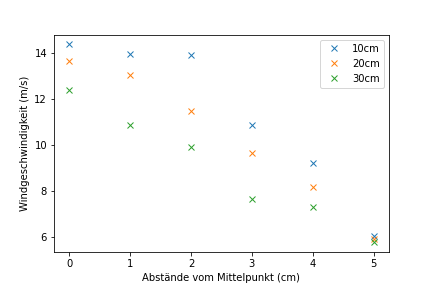
\includegraphics[scale=0.8]{Aeromechanik/Protokoll/fig/Aeromechanik Versuch 1.1.png}
    \caption{Windgeschwindigkeiten für drei verschiedene Abstände vom Gebläse}
    \label{fig:Aeromechanik Versuch 1.1}
\end{figure}

\section{Messung der Windgeschwindigkeit}

In diesem vorbereitenden Versuch geht es darum, die Abhängigkeit zwischen der Drehzahl des Gebläses und der Windgeschwindigkeit zu bestimmen. Um dies für die folgenden Versuche zu nutzen und somit Werte in Abhängigkeit von der Windgeschwindigkeit auszurechnen.

\subsection{Messaufbau}

Um den Versuch zu realisieren, wird der dynamische Druck mithilfe einer kombinierten Sonde gemessen. Wobei hierbei die Differenz zwischen statischem- und Gesamtdruck gemessen wird (vergleiche Demonstrationsversuche). Um nun aus den errechneten Wertepaaren aus dynamischen Druck und Drehzahl Werte für die Windgeschwindigkeit in Abhängigkeit von der Drehzahl aufzustellen, wird die Formel für den dynamischen Druck zu Rate gezogen: 

\begin{equation}
    p_{dyn} = \frac{1}{2} \cdot u^2
    \Rightarrow u = \sqrt{\frac{2p_{dyn}}{\rho}}
\end{equation}

Wobei die positive Wurzel gewählt wird um ein positives Ergebnis für die Geschwindigkeit zu erhalten, außerdem wird für die Dichte, die Dichte von Luft eingesetzt: $\rho = \SI{1.2}{\kg\per\cubic\m}$.

\begin{figure}[h]
    \centering
    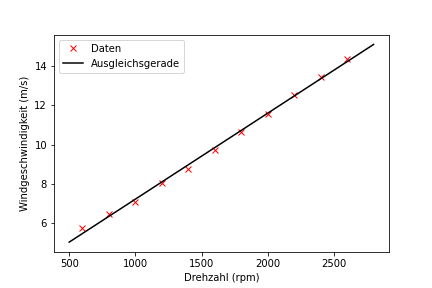
\includegraphics[scale=0.8]{Aeromechanik/Protokoll/fig/Aeromechanik Versuch 1.2.png}
    \caption{Windgeschwindigkeiten für verschiedene Drehzahlen}
    \label{fig:Aeromechanik Versuch 1.2}
\end{figure}

    \chapter{Unströmung von Körpern}
    \section{Rücktrieb und Stirnfläche}

In diesem Versuch soll der Rücktrieb in Abhängigkeit mit der Stirnfläche gemessen werden. Um so einen Teil der Formel für die Kraft in Formel \ref{Kraft} experimentell herzuleiten.

\subsection{Messaufbau}

Um diese Messung zu realisieren werden drei verschieden Große Kreisscheiben in den Luftstrom gebracht und die rücktreibenden Kräfte mit einem Kraftmesser gemessen.

\subsection{Auswertung}

Wir erhalten mit der Messung die Werte in Tabelle \ref{tab:Aufgabe2.1}. Die Werte für den Rücktrieb pro Fläche sind ähnlich, müssten aber unter idealen Bedingungen in der Theorie gleich sein. Allerdings lässt sich diese Abweichung einerseits auf die verschwindend kleine Messreihe zurückführen und auch auf die ungenaue Messmethode, da zum Beispiel Reibung eine große Rolle spielt. Was aber einen wesentlich größeren Effekt hat und auch die gemessene Werte erklären würde, ist die Tatsache, dass es deutlich mehr Verwirbelungen pro Fläche bei kleineren Scheiben im Vergleich zu größeren gibt, was wiederum zu einem größeren Wert für den Rücktrieb pro Fläche führt.

\begin{table}[h]
    \caption{Rücktreibende Kraft für verschieden große Kreisscheiben}
    \centering
    \begin{tabular}{c c c}
    \hline
    Radius Kreisscheibe     & Rücktrieb  & Rücktrieb / Fläche\\
    \hline
    \SI{4}{\centi\metre}     & \SI{0.53}{\newton} & \SI{105.44}{\newton\per\square\metre}\\[5pt]
    \SI{2.8}{\centi\metre}  &   \SI{0.31}{\newton} & \SI{125.86}{\newton\per\square\metre} \\[5pt]
    \SI{2}{\centi\metre}    &   \SI{0.17}{\newton} & \SI{135.28}{\newton\per\square\metre} \\[5pt]
    \hline
    \end{tabular}
    \label{tab:Aufgabe2.1}
\end{table}

\section{Rücktrieb und Strömungsgeschwindigkeit}
\subsection{Messaufbau}

\section{Rücktrieb und Körperform}
\subsection{Messaufbau}

\section{Modellauto}
\subsection{Messaufbau}
    
    \chapter{Strömung am Flügel}
    \section{Auftrieb und Strömungswiderstand}

Dieser Versuch soll die Funktionsweise einer Tragfläche demonstrieren und auch den Einfluss des Anstellwinkels auf den Auftrieb (Kraft nach oben) und Rücktrieb aufzeigen. Mit diesen Werten sollen der beste Anstellwinkel der Tragfläche gefunden werden, was durch das Verhältnis von Auftriebs- und Widerstandskraft ausgedrückt wird. Da dieser Term gleichzeitig bei einem Gleitflug das Verhältnis von zurückgelegter Wegstrecke und Höhenverlust darstellt und somit ein guter Indikator für den besten Anstellwinkel der Tragfläche ist.

\subsection{Messaufbau}

Die Tragfläche wird an einer Auftriebswaage befestig, wobei gleichzeitig durch einen Kraftmesser der Rücktrieb gemessen werden kann. Dann wird mit einer konstante Windgeschwindigkeit von \SI{14.38}{\metre\per\second} und für verschieden Anstellwinkel der Tragfläche der Auftrieb und der Rücktrieb gemessen.

\clearpage

\subsection{Auswertung}

\begin{figure}[h!]
    \centering
    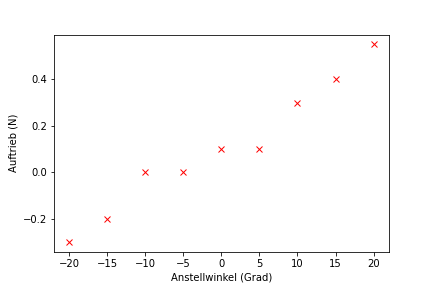
\includegraphics[scale=0.8]{Aeromechanik/Protokoll/fig/Aeromechanik Versuch 3.11.png}
    \caption{Verhältnis von Auftrieb und Anstellwinkel bei konstanter Windgeschwindigkeit}
    \label{fig:Aeoromechanik Versuch 3.11}
\end{figure}

\begin{figure}[h!]
    \centering
    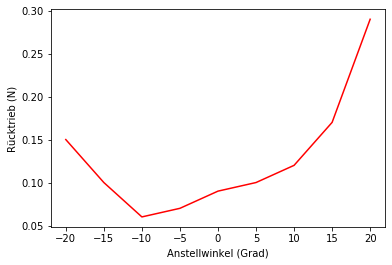
\includegraphics[scale=0.8]{Aeromechanik/Protokoll/fig/Aeromechanik Versuch 3.12.png}
    \caption{Verhältnis von Rücktrieb und Anstellwinkel bei konstanter Windgeschwindigkeit}
    \label{fig:Aeromechanik Versuch 3.12}
\end{figure}

\begin{figure}[h!]
    \centering
    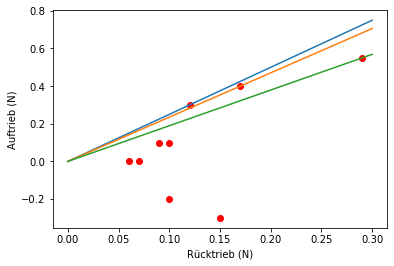
\includegraphics[scale=0.8]{Aeromechanik/Protokoll/fig/Aeromechanik Versuch 3.13.png}
    \caption{Verhältnis von Auftrieb und Rücktrieb bei konstanter Windgeschwindigkeit um die größte Gleitzahl zu finden}
    \label{fig:Aeromechanik Versuch 3.13}
\end{figure}

\section{Druckmessung}
\subsection{Messaufbau}
    
    % appendix for more or less interesting calculations
    \Appendix
    \chapter*{\appendixname} \addcontentsline{toc}{chapter}{\appendixname}
    % to make the appendix appear in ToC without number. \appendixname = 
    % Appendix or Anhang (depending on chosen language)
    \section{Erster Abschnitt des Anhangs}
Dies ist der erste ganz tolle Abschnitt des Anhangs. %\cleardoublepage



    % Bibliography
    \TheBibliography

    % BIBTEX
    % use if you want citations to appear even if they are not referenced to: 
    % \nocite{*} or maybe \nocite{Kon64,And59} for specific entries
    %\nocite{*}
    \bibliographystyle{babalpha}
    \bibliography{lit.bib}

    % THEBIBLIOGRAPHY
    %\begin{thebibliography}{000}
    %    \bibitem{ident}Entry into Bibliography.
    %\end{thebibliography}
\end{document}
